Die bisherigen Ansätze betrachten jeweils nur eine Population. Um die Auswirkungen von Schließungen bestimmter Transportwege zu untersuchen reicht die Betrachtung einer isolierten Population nicht aus. Im Folgenden werden zwei Ansätze zur Modellierung von mehren miteinander agierenden Populationen während einer Infektion untersucht und anschließend darauf aufbauend das Model aus \ref{ssec:spa} auf mehrere Populationen erweitert. Für die eigentliche Erweiterung des Modells wird sich auf eine \emph{SIR}-Modellierung beschränkt und zusätzliche Subpopulationen erst bei Bedarf in Betracht gezogen.
\subsubsection{Verwandte Arbeiten}
\cite{Milne2008} beschreiben in ihrer Arbeit ein Infektionsmodell, mit dem sich die Ausbreitung einer Infektionskrankheit in einer isolierten Stadt beschreiben lässt. Im Gegensatz zu den SIR-Modellen werden in diesem Modell die Individuen direkt simuliert. Innerhalb der Population werden die Individuen in sogenannten \emph{Mixing Groups} zusammengefasst, in denen sich die Individuen untereinander anstecken können. Je nach Interpretation repräsentieren die \emph{Mixing Groups} Haushalte, Schulklassen, Arbeitsplätze oder Krankenhausabteilungen. Jedes Individuum hat dabei eine fest zugeteilte Haushalts- und Beschäftigungsgruppe, zwischen denen im Laufe eines Tages gependelt wird. Dies entspricht dem Arbeits- beziehungsweise dem Schulalltag der Individuen.

Für die Modellierung der Krankheit werden die drei grundlegenden Zustände \emph{infizierbar}, \emph{infiziert} und \emph{immunisiert} eingeführt. Die \emph{Infizierten} unterteilen sich noch zusätzlich in die mit Symptomen und die ohne. Damit ist diese Modellierung einem \emph{SEIR}-Modell ähnlich. Ziel der Arbeit ist es, die Auswirkung von nicht-medikamentösen Maßnahmen bei einer Grippeepidemie zu evaluieren. Die Maßnahmen, darunter auch reduzierter Kontakt innerhalb der Population oder der Schließung von Schulen, zeigten reduzierte Ansteckungsraten.

Zur Veranschaulichung des Modells dient Abbildung \ref{fig:ssec:multipop:milne}, in der eine Population mit Arbeitsplätzen, Schulen und Krankenhäusern dargestellt ist. Die Ansteckung erfolgt nur innerhalb der so genannten ``Mixing Groups''. Die in der Abbildung verwendeten ``Hubs'' dienen nur dem Erhalt der Übersichtlichkeit. Die direkte Simulation von Individuen ist nur in kleinen Populationen praktikabel. Eine größere Population wird aber durch die Wahl einer Stichprobe ebenfalls berechenbar.

\begin{figure}
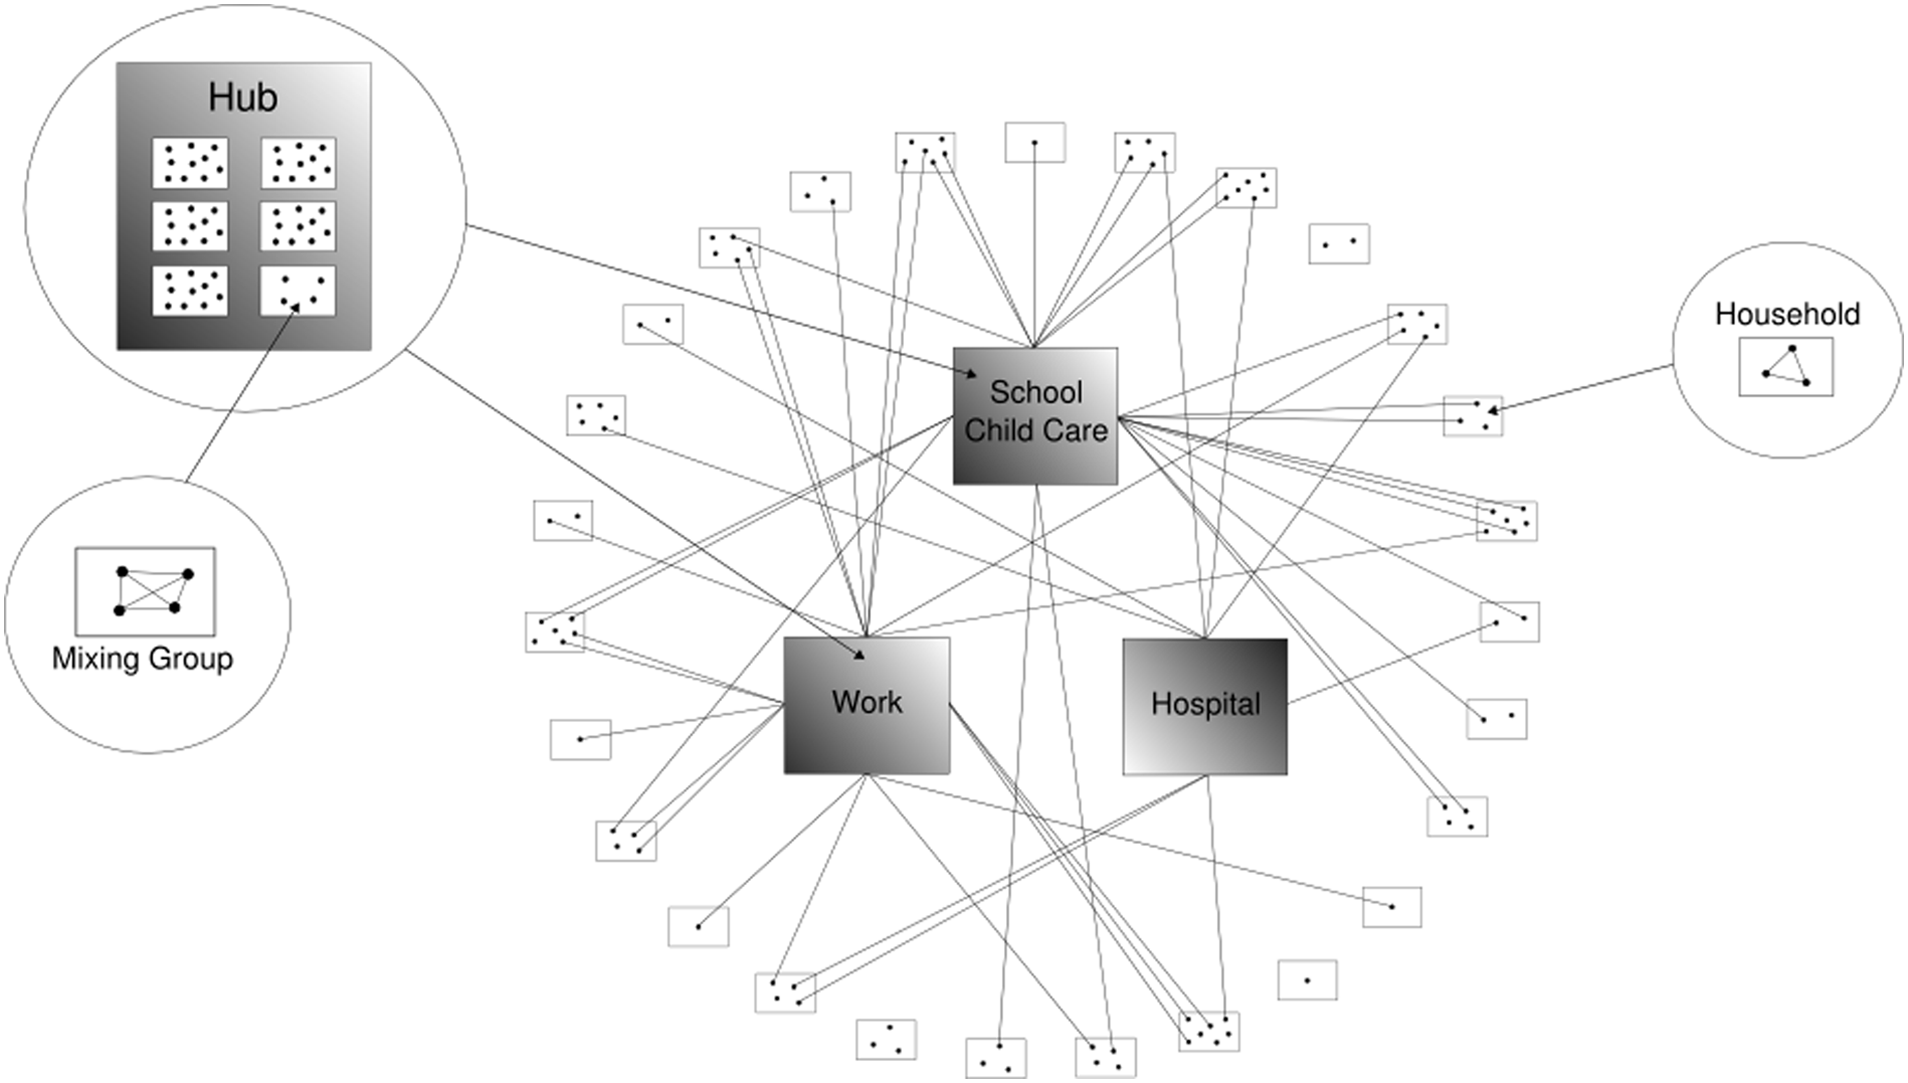
\includegraphics[width=0.8\textwidth]{res/diagramme/milne2008}
\caption{\cite[Figure 1. Idealised household and hub contact network]{Milne2008}}\label{fig:ssec:multipop:milne}
\end{figure}

\cite{Sattenspiel1995} nähert sich der Modellierung von Krankheitsausbreitungen von einer anderen Richtung. Die Basis bildet ein Modell zur Beschreibung von Mobilität zwischen verschiedenen Regionen, in das ein \emph{SIR}-Modell integriert wird. Das Modell beschreibt dabei eine Population, die auf voneinander entfernte Regionen aufgeteilt ist. Die Kontakte zwischen beliebigen Individuen der Gesamtpopulation sind somit nicht mehr zufällig, die zwischen Individuen in der gleichen Region dagegen bleiben es aber. Das Modell lässt sich somit beispielsweise als mehrere verbundene \emph{SIR}-Modelle interpretieren.

Die Mobilität in dem Modell umfasst sowohl einen temporären als auch einen permanenten Austausch von Individuen zwischen den verschiedenen Regionen. Der permanente Austausch ist dabei nicht explizit modelliert, wird aber durch eine entsprechend lange ``Verweildauer'' erreicht. Um die temporäre Verweildauer zu erreichen, muss für jede Bewegung die Menge der bewegten Individuen und die Startregion persistent gemacht werden. Bei schwach partitionierten Populationen, wie sie in der Arbeit untersucht wurden, ist dieser Ansatz durchführbar. Bei stärkerer Partition wächst aber die Menge an Bewegungsinformation exponentiell.
\subsubsection{Vom SIR-Modell zur Netzwerksbasierten Pandemie-Simulation}
Für die Simulation einer Pandemie wird der Netzwerksansatz von \citep{Milne2008} mit der Erweiterung des SIR-Modells von \citep{Sattenspiel1995} kombiniert. 

Sei 
\begin{align}
	P=&\lbrace H, D\rbrace \text{ mit}\label{eq:ssec:multiPop:SIRBegin}\\
	H=&\lbrace S, I, R\rbrace\\
	D=&\lbrace \Delta S= -\lambda SI, \Delta I = \lambda SI - \mu I, \Delta R = \mu I   \rbrace \label{eq:ssec:multiPop:SIREnd}
\end{align}
eine zeitdiskrete SIR-Population. In der folgenden Beschreibung der Pandemie mit einem Netzwerksmodell werden die Subpopulationen der verschiedenen Infektionsstadien mit den Knoten eines gerichteten Netzwerkes identifiziert. Die Knoten enthalten somit auch immer die aktuelle Größe der Subpopulation. Die Kanten werden aus den Änderungsraten gebildet. 

Da die Summe der Subpopulationen inklusive der \emph{R}-Subpopulation zeitinvariant ist gilt, dass es für jeden positiven Summanden in einer Änderungsrate einen betragsmäßig gleichen aber negativen Summanden in einer anderen Änderungsrate gibt. Für die bisher betrachteten \emph{SIR}-Modelle ist dieser Zusammenhang leicht zu sehen:
\begin{align}
	\Delta S & = -\lambda IS & \\
	\Delta I & = \lambda IS & - \mu I \\
	\Delta R & = & \mu I
\end{align}

Die Subpopulation mit dem negativen Summanden in ihrer Änderungsrate wird als Quelle bezeichnet, die mit dem positiven als Senke oder Ziel. So lässt sich die Beziehung zwischen beiden Subpopulationen als Netzwerk mit 2 Knoten und einer gerichteten Kante darstellen (siehe Abbildung \ref{fig:ssec:multiPop:simpleDirectedEdge}) und als ``Abwandern'' von Individuen aus der Quell-Subpopulation in die Senken-Subpopulation interpretieren. Die Menge an Individuen, die entlang der Kante abwandert, nennen wir das \emph{Volumen} der Kante. 

\begin{figure}
\begin{center}\begin{tikzpicture}[->,>=stealth',shorten >=1pt,auto, node distance=3cm]
	\node[state] (S)				{S};
	\node[state] (I) [right of=S]	{I};
	
	\path (S) edge node {$\lambda SI$} (I);
\end{tikzpicture}\end{center}
\caption{Beispiel einer Quelle-Senke Relation zwischen zwei Subpopulationen.}\label{fig:ssec:multiPop:simpleDirectedEdge}
\end{figure}

Mit der soeben beschriebenen Transformation lässt sich das bekannte \emph{SIR}-Modell nun als Netzwerk darstellen. Für das \emph{SIR}-Modell in Gleichung \ref{eq:ssec:multiPop:SIRBegin} - \ref{eq:ssec:multiPop:SIREnd} wird das Netzwerk in Abbildung \ref{fig:ssec:multiPop:SIRNet} dargestellt.

\begin{figure}
\begin{center}
\begin{tikzpicture}[->,>=stealth',shorten >=1pt,auto, node distance=3cm]
	\node[state] (S)				{S};
	\node[state] (I) [right of=S]	{I};
	\node[state] (R) [right of=I]	{R};
	\path 	(S) edge node {$\lambda SI$}	(I)
			(I) edge node {$\mu I$}			(R);
\end{tikzpicture}
\end{center}
\caption{Netzwerkdarstellung von Gleichung \ref{eq:ssec:multiPop:SIRBegin} - \ref{eq:ssec:multiPop:SIREnd}}\label{fig:ssec:multiPop:SIRNet}
\end{figure}

Die Erweiterung der Modellierung auf multiple, miteinander interagierende Populationen wird nun mit der Erweiterung des Netzwerkes um weitere Populationen sowie zusätzlichen Kanten zwischen den Populationen erreicht. Mit der Motivation der Modellierung im Hinterkopf wird im Folgenden von einem \emph{SEIR}-Modell ausgegangen. In \cite{Sattenspiel1995} wird eine Interaktion zwischen den Populationen uniform modelliert. Jede Subpopulation hat die gleiche Reiserate. Dieser Ansatz vereinfacht die Realität aber stark. Je nach zu simulierender Krankheit sind Infizierte mit Symptomen (Subpopulation \emph{I}) körperlich nicht mehr in der Lage zu reisen oder werden, auf Grund ihrer offensichtlichen Krankheit, auf gewissen Transportwegen nicht mehr befördert. Dies gilt beispielsweise für Flugzeuge oder Schiffe, bei denen die Passagiere gemeinsam auf einem engen, abgeschlossenen Raum miteinander interagieren. Unter dieser Prämisse wäre ein \emph{SIR}-Modell zur Beschreibung von Pandemien nicht sinnvoll. Es würde nur ein Austausch zwischen den verschiedenen \emph{S}-Populationen stattfinden und Infizierte würden keine Nachbarpopulationen kontaminieren.  Durch die Hinzunahme einer \emph{E}-Population, in der die nichtsymptomatischen Infizierten zusammengefasst werden, wird das Kontaminationsproblem gelöst, da diese Individuen die Krankheit durch alle Transportwege in andere Populationen tragen können. 

Für das Populationsnetzwerk bedeutet dies, dass jeweils zwischen allen \emph{S}-Subpopulationen und allen \emph{E}-Subpopulationen Kanten dem Netzwerk hinzugefügt werden, die den Fluss zwischen den Subpopulationen beschreiben. Für ein besseres Verständnis wird im Folgenden zwischen inneren und äußeren Kanten unterschieden. Die inneren Kanten beschreiben die Kanten innerhalb einer Population und die äußeren die Interaktion zwischen den Populationen. Für die weitere Modellierung einer Pandemie wird angenommen, dass die Infizierte mit Symptomen nicht reisen. Zudem werden die Interaktionen zwischen den \emph{R}-Subpopulationen nicht modelliert, da diese für die Betrachtung einer Krankheit keine Bedeutung mehr haben und hauptsächlich als ``Endlager'' für Individuen dienen, die nicht mehr durch die Krankheit beeinflusst werden können (zum Beispiel durch Immunisierung oder Tod). Für zwei \emph{SEIR}-Populationen $P$ und $P'$ ist das Netzwerk in Abbildung \ref{fig:ssec:multiPop:2interactingSEIR} dargestellt. 
\begin{figure}
\begin{center}
\begin{tikzpicture}[->,>=stealth',shorten >=1pt,auto, node distance=3.5cm]
	\node[state] (S)				{S};
	\node[state] (E) [right of=S]	{E};
	\node[state] (I) [right of=E]	{I};
	\node[state] (R) [right of=I]	{R};
	\node[state] (S')[below of=S]	{S'};
	\node[state] (E')[below of=E]	{E'};
	\node[state] (I')[below of=I]	{I'};
	\node[state] (R')[below of=R]	{R'};
	\path 	(S)	edge node {$\lambda SE + \beta SI$} 	(E)
				edge [bend left] node {$T^{P,P'}$}					(S')
			(E)	edge node {$\gamma E$}					(I)
				edge [bend left] node {$T^{P,P'}$}					(E')
			(I)	edge node {$\delta I$}					(R)
			(S')edge node {$\lambda S'E' + \beta S'I'$}(E')
				edge [bend left] node {$T^{P',P}$}					(S)
			(E')edge node {$\gamma E'$}					(I')
				edge [bend left] node {$T^{P',P}$}					(E)
			(I')edge node {$\delta I'$}					(R');
	
\end{tikzpicture}
\end{center}
\caption{Netzwerk für zwei interagierende \emph{SEIR}-Populationen mit gleichen Übergangskoeffizienten}\label{fig:ssec:multiPop:2interactingSEIR}
\end{figure}

Stünde in diesem Beispiel jede Population für ein Land, würden die gleichen Übertragungsfaktoren ($\alpha, \beta, \gamma, \delta$) auf ähnliche Strukturen in der Behandlung von Krankheiten hinweisen. 

In Abbildung \ref{fig:ssec:multiPop:2interactingSEIR} wird jeweils ein Faktor für die äußeren Kanten von $P$ nach $P'$ ($\tau$) und einer für die Gegenrichtung ($\pi$) verwendet. Dieser Faktor wird im Folgenden als Reisefaktor bezeichnet und ist zwischen zwei Populationen für alle Subpopulationen gleich. Da in unserem Modell nur symptomfreie Individuen reisen, haben Individuen der \emph{E}-Subpopulation keinen Grund weniger zu reisen als die Individuen der \emph{S}-Subpopulation. Eine Verallgemeinerung auf subpopulationsabhängige Reisefaktoren ist jedoch nicht ausgeschlossen. 

Das Volument einer Reisekante von Population $A$ nach Population $B$ wird beschrieben mit
\begin{align}
	T^{A,B} = T^{A,B}_{s} \cdot T^{A,B}_{d}. 
\end{align}
$T^{A,B}_s$ beschreibt dabei den Einfluss statischer Gegebenheiten auf das Reisevolumen und $T^{A,B}_d$ eine Skalierung, die die dynamischen Gegebenheiten darstellt. Die Gründe für den Austausch von Individuen zwischen zwei Populationen sind im Allgemeinen Migration, Tourismus und Beruf. Im Falle einer tötlichen Krankheit kann auch noch die Flucht vor dieser Krankheit ein Reisegrund sein. Verbleibt ein Individuum in der Zielpopulation, also im Falle von Migration oder Flucht, ist die Integration dieses Falles in das \emph{SIR}-Modell einfach, da es ähnlich zum Übergang von einem Krankheitszustand zum nächsten. Im Falle von Tourismus und Beruf, in dem die Individuen periodisch zu ihrer Startpopulation zurückkehren, ist die Integration hingegen schwierig. Die \emph{SIR}-Modelle sind gedächtnislos; die Berechnung des nächsten Simulationsschrittes ist nur abhängig von den aktuellen Größen der Subpopulationen. Diese Eigenschaft ist sowohl für den Schuleinsatz als auch allgemein für eine Simulation von Vorteil. So ist beispielsweise der benötigte Speicherplatz für die Berechnung eines Simulationsschrittes natürlich geringer. Vor allem mit dem Schuleinsatz im Fokus soll diese Eigenschaft erhalten bleiben. Um die Gedächtnislosigkeit zu erhalten und gleichzeitig Tourismus und Pendelberufe zu simulieren, wäre folgender Ansatz möglich.

Jede Population \emph{P} erhält für jede reisende Subpopulation $Y$ (in unserem Fall \emph{S} und \emph{E}) und jede besuchende Nachbarpopulation \emph{X} eine zusätzliche Subpopulation $P.Y^X_T$, die als Ziel für alle Reisenden aus $X$ nach $P$ dient. Somit \emph{konserviert} man die Information, wieviele Individuen im aktuellen Zeitschritt von \emph{X} nach \emph{P} gereist sind. $P.Y^X_T$ erhält eine Reisekante zurück nach $X.Y$ mit einem Volumenfaktor von 1. Alle Reisenden kehren also einen Simulationsschritt nach Ankunft wieder in ihr Ursprungsland zurück. Die inneren Kanten müssen dahingehend angepasst werden, dass die Individuen in den Reisesubpopulationen in die Kantenvolumen eingerechnet werden. Weiterhin müssen innere Kanten, also Krankheitszustandsübergange, zwischen den Reisepopulationen hinzugefügt werden, um eine Ansteckung im Zielland zu ermöglichen. So sind dann Tourismus und Berufspendeln gedächtnislos in das Modell integriert. Nur ``erkauft'' man sich diese Integration bei $n$ Populationen mit insgesamt $2n^2-2n$ zusätzlichen Subpopulationen und wenn im weiteren Verlauf der Arbeit die Reisewege noch nach Art aufgeteilt werden vervielfacht sich diese Zahl weiter. Dieser quadratische Anstieg an Subpopulationen macht das Modell unhandlich bis unbrauchbar bei großen Simulationen. Möchte man beispielsweise den Verlauf des letzten Ebolaausbruches in ganz Afrika (54 Länder) simulieren erhält man in dem von uns beschriebenen \emph{SEIHFRD}-Modell $378$ Subpopulationen. Wendet man nun die Tourismuserweiterung darauf an, erhält man in jeder Population $2\cdot 53$ Subpopulationen dazu, was zu insgesamt $6102$ Subpopulationen führt. 

Dieser Zusatz an zu verwaltenden Subpopoulationen erscheint als zu hoch für den modellierten Aspekt, weswegen er in das hier beschriebene Modell nicht aufgenommen wird. Es wird also nur die Migration und die Flucht vor einer Epidemie modelliert. Beginnen wir mit der Migration. 

Das Migrationsvolumen wird berechnet mit
\begin{align}
	T^{A,B}_s=T^{A,B}_{Mig} = f_{att}(A,B)\cdot M_A.
\end{align}
Dabei ist $f_{att}(A,B) \in [0,1]$ der Anteil der emigrierenden Individuen aus $A$ nach $B$. Für alle Populationen $A$ gilt dabei immer
\begin{align}
	\sum\limits_{X \in H \& X\neq A} f_{att}(A,X) = 1\label{eq:ssec:multiPop:constAtt}
\end{align}
$f_{att}$ beschreibt die \emph{Attraktivität} der Population $B$ aus Sicht von $A$. Im Falle von Migration wird sich dies primär auf den Lebensstandard innerhalb der Population beziehen. Seien $L_A$ und $L_B\in \mathbb{N^+}$ Repräsentationen des Lebensstandards in $A$ und $B$. Wir definieren dann $f_{att}$ wie folgt:
\begin{align}
		f_{att} :& \mathbb{N}\times \mathbb{N}\times H \rightarrow  [0,1]\\
			 & (L_A,L_B,A)\longmapsto		c_A\cdot\frac{L_B}{L_A}& \text{und}\nonumber\\
		c_A = & \left( \sum\limits_{B\in H, B\neq A} \frac{L_B}{L_A}\right)^{-1}&
\end{align}
Durch die Wahl von $c_A$ wird die Forderung in Gleichung \ref{eq:ssec:multiPop:constAtt} immer erfüllt.

Der Faktor $M_A$ beschreibt den Anteil der Bevölkerung von $A$, der in der Lage ist zu migrieren. Über den Zeitraum der Simulation wird dieser als konstant angenommen. Da Tourismus und internationales Berufspendeln ausgenommen sind, ist der Migragrationsfaktor bereits der statische Reisefaktor $T^{A,B}_s$. Somit sind die Gründe modelliert, aus denen ein Individuum von einer Population in eine andere übersiedeln möchte. Der Einfluss einer Epidemie ist dabei aber noch unberücksichtigt. 

Modelliert man eine gefährliche Krankheit wie das Ebolavirus, wirkt sich deren Verbreitung innerhalb von Populationen auf das Reiseverhalten aus. Wütet eine solche Krankheit in der eigenen Population wird sich ein größerer Anteil der Population eher für die Migration entscheiden, als dies ohne Epidemie der Fall wäre. Gleichzeitig wird eine solche Population auch weniger Immigration erfahren, da sich Individuen aus weniger betroffenen Populationen eher nicht der Gefahr einer Infektion aussetzen. Wir definieren den dynamischen Reisefaktor als
\begin{align}
	T^{A,B}_d =& f_{inf}(i_A,i_B, \sigma)&\text{mit}\\
	f_{inf}(i_A,i_B,\sigma) \in& \mathbb{R}^+&\text{der Infektionseinschätzung von A bzgl. B,}\label{eq:ssec:multiPop:infRisk}\\
	i_X =& \frac{|X.I|}{|X|}&\text{dem Infektionsquotienten und}\\
	\sigma \geq&1 & \text{die Schwere der Krankheit}\label{eq:ssec:multiPop:severity}
\end{align}
In dem erweiterten \emph{SEIHFRD}-Modell (siehe Abbildung \ref{fig:ssec:model}) berechnet sich der der Infektionsquotient via 
\begin{align}
	i_X = \frac{|X.I|+|X.H|}{|X| - |X.D|}.
\end{align}
Der Infektionsquotient beschreibt die Wahrnehmung der Ausbreitung einer Krankheit innerhalb einer Population. Die \emph{Infektionseinschätzung} $f_{inf}$ von $A$ bezüglich $B$ hängt von den Infektionsquotienten von $A$ und $B$ ab. Ist $i_A = i_B$, wird die Infektion innerhalb der Zielpopulation als so schwer wie in der Ausgangspopulation wahrgenommen, wirkt die Krankheit weder beschleunigend noch bremsend auf die Migration. Es ist somit $f_{inf}(i_A,i_B,\sigma)=1$, unabhängig von der schwere der Krankheit. $f_{inf}$ kann beliebig komplex gewählt werden. Dabei sollten jedoch die folgenden Eigenschaften gelten:
\begin{align}
	\forall x, y \in [0,1], \sigma \geq 1 & \nonumber\\
		& f_{inf}(x,x,\sigma) = 1\\
		& f_{inf}(x,y,\sigma) \geq 0\\
		& x < y \Rightarrow f_{inf}(x,y,\sigma) < 1 \label{eq:ssec:multiPop:infRisklow}\\
		& x > y \Rightarrow f_{inf}(x,y,\sigma) > 1 \label{eq:ssec:multiPop:infRiskhigh}
\end{align}
Die Eigenschaft aus Gleichung \ref{eq:ssec:multiPop:infRisklow} beschreibt die Dämpfung der Migration, wenn in der Zielpopulation die zu simulierende Krankheit bereits vebreiteter ist, als in der Ausgangspopulation. Gleichung \ref{eq:ssec:multiPop:infRiskhigh} beschreibt analog die Migration in eine \emph{gesündere} Zielpopulation.

Für dieses Modell wählen wir
\begin{align}
	f_{inf} :& [0,1]\times [0,1] \times \mathbb{R}^+ \rightarrow  \mathbb{R}^+\\
			 & (i_A,i_B,\sigma)\longmapsto								\begin{cases}c_{inf}&\text{, wenn } i_B = 0 \vee \frac{i_A}{i_B} > c_{inf} \\\left( \frac{i_A}{i_B}\right)^\sigma &\text{, sonst}\end{cases}\nonumber			  
\end{align}
Für den Fall $i_B$ wird eine Konstante $c_inf$ angegeben, die gleichzeitig als obere Schranke fungiert. Eine obere Schranke ist auch notwendig, denn für $i_A >0$ fest und $i_B\rightarrow 0$ gilt $\frac{i_A}{i_B}\rightarrow \infty$. Innerhalb des Modells würde dies bedeuten, dass bereits aus einer nur leicht infizierten Population alle Individuen innerhalb eines einzelnen Zeitschrittes in eine völlig gesunde Population ``fliehen'' würden. Für den weiteren Verlauf wird $c_{inf} = 2$ gesetzt. 

Der Reisefaktor wird auf alle Subpopulationen unverändert angewandt. Man erhält damit für zwei \emph{SEIR}-Populationen das in Abbildung \ref{fig:ssec:multiPop:travelSEIR} dargestellte Netzwerk.
\begin{figure}
\begin{center}
\begin{tikzpicture}[->,>=stealth',shorten >=1pt,auto, node distance=3.5cm]
	\node[state] (AS)				{A.S};
	\node[state] (AE) [right =6cm of AS]{A.E};
	\node[state] (AI) [right =1cm of AE]{A.I};
	\node[state] (AR) [right =1cm of AI]{A.R};
	\node[state] (BS)[below of=AS]	{B.S};
	\node[state] (BE)[below of=AE]	{B.E};
	\node[state] (BI)[below of=AI]	{B.I};
	\node[state] (BR)[below of=AR]	{B.R};
	\path 	(AS)	edge 				node {}						(AE)
					edge [bend left] 	node {$A.S \cdot T^{A,B}$}	(BS)
			(AE)	edge 				node {}						(AI)
					edge [bend left] 	node {$A.E\cdot T^{A,B}$}	(BE)
			(AI)	edge 				node {}					 	(AR)
			(BS)	edge			 	node {}						(BE)
					edge [bend left] 	node {$B.S\cdot T^{B,A}$}	(AS)
			(BE)	edge 				node {}						(BI)
					edge [bend left] 	node {$B.E\cdot T^{B,A}$}	(AE)
			(BI)	edge 				node {}						(BR);
	
\end{tikzpicture}
\end{center}
\caption{Netzwerk für zwei interagierende \emph{SEIR}-Populationen mit Reisevolumina}\label{fig:ssec:multiPop:travelSEIR}
\end{figure}
Die so definierten Reisekanten umfassen immer den kompletten Strom von Individuen von einer Population in eine andere. Für die Ausbreitung von Krankheiten kann es aber interessant sein, zu wissen, welche Wege ein Individuum nehmen kann, um in eine Population einzureisen. Einer Person mit offensichtlichen Krankheitszeichen wird beispielsweise die Reise mit einem Flugzeug verwehrt, während die Reise mit dem Automobil über offene Grenzen völlig unkontrolliert erfolgt. Wir legen zudem fest, dass die \emph{bodengebundenen} Transportmittel wie Auto oder Zug Individuen nur in die geographisch benachbarten Populationen transportieren können. Der Transport via Flugzeug kann dagegen potentiell von jeder Population in jede andere erfolgen. 

Die bisher modellierte Reisekante wird also in bodengebunden Verkehr und in Flugverkehr aufgeteilt. Die quantitative Aufteilung ist abhängig von lokalen Gegebenheiten, wie dem Durchschnittseinkommen, der Verbreitung von Flughäfen und natürlich dem Kostenverhältnis zwischen einer Auto-/Zugfahrt und einem Linienflug. Dabei sind Durchschnittseinkommen, Flughafendichte oder das Kostenverhältnis noch nicht als Information im Modell vorhanden. Deren Hinzunahme führt zu einer erhöhten Komplexität des Modells. Aus diesem Grund wird auf eine parametrisierte Darstellung der quantitativen Aufteilung der Reisekanten verzichtet und der Anteil am Reisevolumen für jede Reisekante direkt angegeben. Aus Konsistenzgründen gilt, dass die Summe der Anteile aller aufgespalteten Reisekanten von einem Startknoten zu einem Zielknoten immer gleich $1$ sein muss. Ebenso sind mehrere Kanten der gleichen Fortbewegungsart von einem Startknoten zu einem Zielknoten redundant und werden deswegen nicht modelliert. Zwischen zwei Knoten kann es für jeden Fortbewegunstyp also nur eine Reisekante geben. 